\documentclass[a4paper]{scrartcl}
\usepackage{makecell}
\usepackage{multicol}
\usepackage{graphicx}
\usepackage{anysize}
\usepackage{amsmath}
\usepackage{kpfonts}
\usepackage{tabularx}
\usepackage{hyperref}
\usepackage{listings}
\usepackage{color}

\marginsize{25mm}{25mm}{25mm}{25mm}
%---Code-Editor Config ------------------------%
\definecolor{dkgreen}{rgb}{0,0.6,0}
\definecolor{gray}{rgb}{0.5,0.5,0.5}
\definecolor{mauve}{rgb}{0.58,0,0.82}
\definecolor{backcolour}{rgb}{0.95,0.95,0.92}
\lstset{basicstyle=\ttfamily}
\lstset{literate=%
  {Ö}{{\"O}}1
  {Ä}{{\"A}}1
  {Ü}{{\"U}}1
  {ß}{{\ss}}1
  {ü}{{\"u}}1
  {ä}{{\"a}}1
  {ö}{{\"o}}1
  {é}{{\"AC}}1
  {€}{{\"AC}}1
}
\lstset{
	language=Python,				% the language of the code
	basicstyle=\footnotesize,			% the size of the fonts that are used for the code
	numbers=left,					% where to put the line-numbers
	numberstyle=\tiny\color{gray},		% the style that is used for the line-numbers
	stepnumber=1,					% the step between two line-numbers. If it's 1, each line will be numbered
	numbersep=5pt,				% how far the line-numbers are from the code
	backgroundcolor=\color{white},		% choose the background color. You must add \usepackage{color}
	showspaces=false,				% show spaces adding particular underscores
	showstringspaces=false,			% underline spaces within strings
	showtabs=false,				% show tabs within strings adding particular underscores
	frame=single,					% adds a frame around the code
	rulecolor=\color{black},			% if not set, the frame-color may be changed on line-breaks within not-black text (e.g. commens (green here))
	tabsize=2,						% sets default tabsize to 2 spaces
	captionpos=b,					% sets the caption-position to bottom
	breaklines=true,                			% sets automatic line breaking
  	breakatwhitespace=false,       		% sets if automatic breaks should only happen at whitespace
  	title=\lstname,        % show the filename of files included with \lstinputlisting; % also try caption instead of title
  	keywordstyle=\color{blue},          	% keyword style
  	commentstyle=\color{dkgreen},       	% comment style
  	stringstyle=\color{mauve},         		% string literal style
  	escapeinside={\%*}{*)},            		% if you want to add LaTeX within your code
  	morekeywords={*,...}              		% if you want to add more keywords to the set
}

%Header and Footer -----------------------%
\usepackage[headsepline]{scrlayer-scrpage}
\pagestyle{scrheadings}
\clearpairofpagestyles
%\setlength{\headheight}{40.8pt}
\setlength{\headheight}{56pt}
\ihead{IRTM\\ Wi 20/21\\ Assigment 1} 
\ohead{
    Alberto Saponaro - saponaroalberto97@gmail.com\\
    Walter Väth - walter.vaeth@gmail.com\\
    Chong Shen - st143575@stud.uni-stuttgart.de\\
    Xin Pang - st145113@stud.uni-stuttgart.de
}
\ofoot{\pagemark}

%-----------------------------------------------%
%  BEGIN                                        %
%-----------------------------------------------%
\begin{document}
    
\section*{Task 1}
\subsection{Subtask 1}
\begin{center}
    $w_{t,d}=(1+\log tf_{t,d})*\log \frac{N}{df_t}$
\end{center}
\begin{itemize}
    \item $w_{pens, d_1} = (1+\log 1) * \log \frac{3}{1} \approx  1,1$
    \item $w_{pens, d_2} = $ not in the doc
    \item $w_{pens, d_3} = $ not in the doc
    \item $w_{write, d_1} = (1+\log 1) * \log \frac{3}{3} = 0$
    \item $w_{write, d_2} = (1+\log 1) * \log \frac{3}{3} = 0$
    \item $w_{write, d_3} = (1+\log 1) * \log \frac{3}{3} = 0$
    \item $w_{on, d_1} = (1+\log 1) * \log \frac{3}{3} = 0$
    \item $w_{on, d_2} = (1+\log 1) * \log \frac{3}{3} = 0$
    \item $w_{on, d_3} = (1+\log 1) * \log \frac{3}{3} = 0$
    \item $w_{paper, d_1} = (1+\log 2) * \log \frac{3}{3} = 0$
    \item $w_{paper, d_2} = $ not in the doc
    \item $w_{paper, d_3} = (1+\log 1) * \log \frac{3}{3} = 0$
    \item $w_{pencils, d_1} = $ not in the doc
    \item $w_{pencils, d_2} = (1+\log 1) * \log \frac{3}{1} \approx 1,1$
    \item $w_{pencils, d_3} = $ not in the doc
    \item $w_{envelope, d_1} = $ not in the doc
    \item $w_{envelope, d_2} = (1+\log 1) * \log \frac{3}{1} \approx 1,1$
    \item $w_{envelope, d_3} = $ not in the doc
    \item $w_{ballpens, d_1} = $ not in the doc
    \item $w_{ballpens, d_2} = $ not in the doc
    \item $w_{ballpens, d_3} = (1+\log 1) * \log \frac{3}{1} \approx 1,1$
\end{itemize}

\subsubsection*{Subtask 2}


\pagebreak
\subsection*{Task 3}

\begin{itemize}
    \item $Precision = \frac{TPs}{TPs+FPs}$
    \item $Recall = \frac{TPs}{TPs+FNs}$
\end{itemize}

\begin{center}
    \begin{tabular}{@{}llll@{}}
    \hline
    \textbf{k} & \textbf{Result Set}           & \textbf{Precision} & \textbf{Recall} \\ \hline
    1          & 127                           & 1.0                & 0.2             \\
    2          & 127, 9                        & 0.5                & 0.2             \\
    3          & 127, 9, 10                    & 0.33               & 0.2             \\
    4          & 127, 9, 10, 2                 & 0.5                & 0.4             \\
    5          & 127, 9, 10, 2, 35             & 0.4                & 0.4             \\
    6          & 127, 9, 10, 2, 35, 32         & 0.33               & 0.4             \\
    7          & 127, 9, 10, 2, 35, 32, 41     & 0.43               & 0.6             \\
    8          & 127, 9, 10, 2, 35, 32, 41, 64 & 0.5                & 0.8             \\ \hline
    \end{tabular}
    
    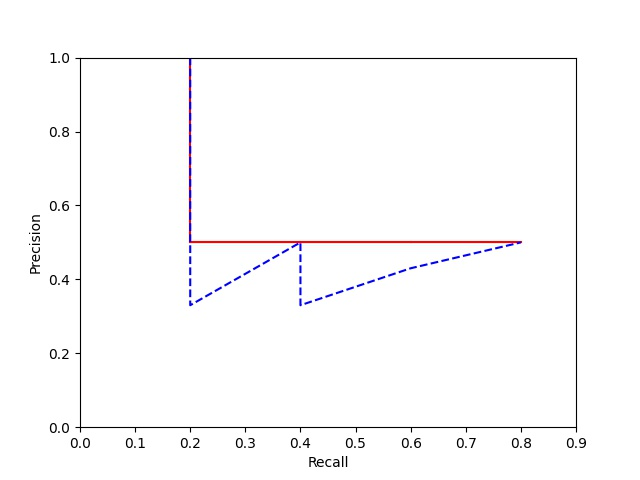
\includegraphics[width=.7\textwidth]{img/fig.jpg}
\end{center}




\end{document}